\chapter{Implementations}
\label{Implementations}
This chapter will follow up on (TODO: MAYBE INSERT SOMETHING HERE) and will introduce the reader on the different implementations done within the scope of the thesis. It will start by introducing the reader with the basics of the algorithm and introduce the strategies and techniques used for implementing a sequential version, a parallel version allowing to price one option per thread, another parallel version allowing to price multiple options per thread and finally exploitation of full parallelism. 

\section{Algorithm and intuition}
\label{section:algorithm_and_intuition}
While it is possible to start from a provided code base and apply various transformations to make it parallel and improve its performance, in order to achieve maximum parallelization efficiency, it is necessary to have a deep understanding of the algorithm itself. The book by John Hull\cite{ofod} provides a solid background on the topic, describing the mechanics of interest rates, markets, the need for binomial trees and how that has led to the use of trinomial trees. Chapter 30 further narrows the topic of using trinomial trees as a numerical method and introduces a step by step walk-through of applying the algorithm on a basic example. While some of the calculation details are omitted in the book, the authors provide references to previous articles\cite{npfits}\cite{uhwirt}, where they explain them. 

It is worth mentioning that the construction of the tree is a numerical method, but the example in the book is simplified by using analytic formulas, as the authors cut the trinomial tree at a certain time step and introduce a set of mathematical functions to calculate option values. While this simplification will give sufficiently good results in many cases, constructing the entire tree and using all of the time steps is naturally more precise, even though computationally harder. All the implementations of our project will be focused on the numerical approach only - constructing the entire tree.

The algorithm consists of two general steps. The first (forward propagation along the tree) is the construction of the trinomial tree in order to obtain a list of alpha values for each time step. These alphas are later used in the second step (backward propagation along the tree) to fit the bond prices and obtain the option value back at the root node of the tree. The input fed to the algorithm consists of a list of options, as for each option the information provided is its strike price, maturity, time step length, reversion rate\footnote{denoted as $a$ - determines the relative volatilities of long and short rates\cite[pg.9]{npfits}} and volatility\footnote{denoted as $\sigma$ - determines the overall level of volatility \cite[pg. 9]{npfits}}. The output is a list of option values for each inputted option. 

The following sub-chapters are focused primarily on the intuition behind the algorithm, with the sole purpose to provide the reader with a general overview of it. For this reason, many of the details and formulas of calculating specific values have been omitted, as they are thoroughly described in the book and the articles by Hull and White. As the model is best understood visually, we have included some of the supplementary images from the Hull and White book in order to support our algorithm explanation. 

\subsection{Forward propagation}
The forward propagation itself consists of two stages. Furthermore, each stage computes different values on the same tree. While the tree height can grow indefinitely, depending on the number of time steps, Hull and White limit the width of the tree (TODO: FOR NO APPARENT REASON !!!), by setting $j_{min}$ and $j_{max}$\footnote{As the tree is 2 dimensional, in order to find and operate on every single node, it is necessary to use both its x and y coordinates, in this case denoted $i$ and $j$ respectively.} defining the maximum span of its width (where the root is located on $j=0$)

\subsubsection{Stage 1}
The first stage aims to construct a tree for a variable $R^*$ that is initially 0 and follows the process $dR^*=-aR^*dt + \sigma dz$ which is symmetrical about $R^*=0$\cite[pg.698-699]{ofod}. Together with $R^*$, $p_u$, $p_m$ and $p_d$ are calculated to match the respective up, mid and down probabilities that match the expected change and variance of the change in R over the next interval $\triangle t$. Since the width of the tree is limited between $j_{min}$ and $j_{max}$, some of the branching is calculated differently, thus $p_u$, $p_m$ and $p_d$ depend on the node position. Naturally the tree construction happens iteratively, node by node, starting from the root. In the end of the stage, this first tree will always have a symmetrical shape similar\footnote{Note that the width and height of the tree may differ based on the number of time steps and the maturity of the financial instrument} to fig.\ref{treeconststage1}. 
\begin{figure}[H]
	\centering
	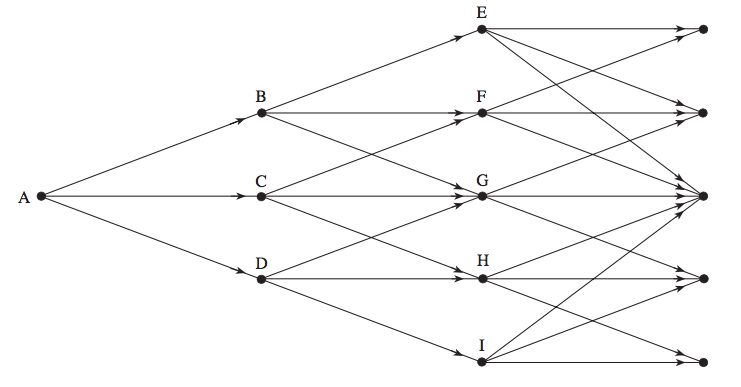
\includegraphics[width=0.8\textwidth]{img/treeconststage1.png}
	\caption{Example of the trinomial tree for $R^*$. Source: figure 30.8 \cite[pg. 699]{ofod}}
	\label{treeconststage1}
\end{figure}

Some of the important properties of this tree include first of all the symmetry. The probabilities on the lower part of the tree will be the negative of the probabilities on the upper part of the tree, e.g. probability that node A reaches node D is minus the probability of node A reaching node B. Furthermore, also due to symmetry, all unique probabilities can be stored in an array of size the width of the tree, e.g. the probability of node A reaching node B is the same as the probability of node C reaching node F and so on. Probabilities are used both in stage 2 of the forward propagation, but also in the backward propagation, thus it is necessary to preserve them to the end. Last but not least, the way probabilities are calculated is different on $j_{min}$ or $j_{max}$, because of the difference in branching. 

\subsubsection{Stage 2}
In this stage, the rates at each node in the tree at each time step are shifted up by an amount - $\alpha$, chosen so that the revised tree correctly prices discount bonds \cite[pg. 6]{uhwirt}. This is done by defining $Q_{i,j}$ as the present value of a security that pays off \$1 if node (i, j) is reached and 0 otherwise. The starting point is to set $Q_{0,0}=0$ and $\alpha_0$ to the interest rate at time $\triangle t$.$Q$s at the next time step are then calculated by using the generalized formula \cite[pg.705]{ofod}:  
\begin{equation}
\begin{gathered}
\begin{aligned}
Q_{m+1, j} = \sum_k Q_{m,k}q(k,j)exp[-(\alpha_m+k\triangle r)\triangle t]
\nonumber
\end{aligned}
\end{gathered}
\end{equation}
Supposing that we are starting on step $m$, to calculate the $Q$s on step $m+1$, we need to have the alpha on step $m$. Furthermore, once the $Q$s on step $m+1$ have been calculated, they are used to also find the alpha on $m+1$ later. This leads to the conclude that alphas and $Q$s are interrelated on each time step. Alphas are calculated using the generalized formula \cite[pg.703]{ofod}:
\begin{equation}
\begin{gathered}
\begin{aligned}
\alpha_{m} = \dfrac{\sum_{j=-n_m}^{n_m} Q_{m,j}e^{-j\triangle r\triangle t} - \ln{P_{m + 1}}}{\triangle t}
\nonumber
\end{aligned}
\end{gathered}
\end{equation}
At the end of this stage, the new tree will have a similar shape to the one shown in fig. \ref{treeconststage2}. 
\begin{figure}[H]
	\centering
	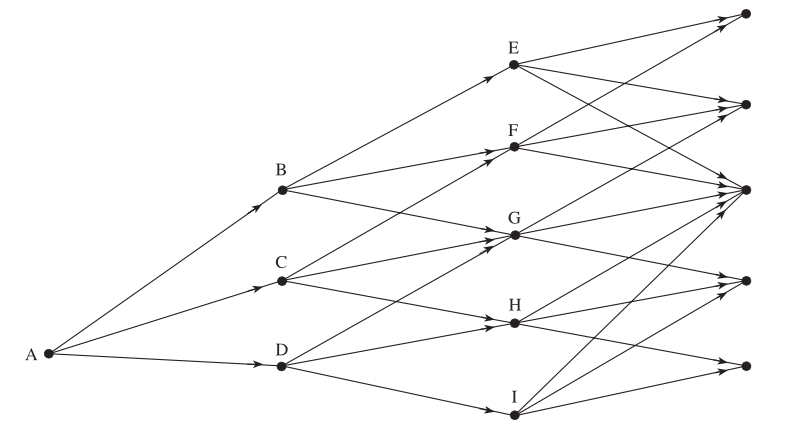
\includegraphics[width=0.8\textwidth]{img/treeconststage2.png}
	\caption{Example of the trinomial tree for $R$. Source: figure 30.9 \cite[pg. 702]{ofod}}
	\label{treeconststage2}
\end{figure}
An important observation here is that the only outcome of this tree that is used in the backward propagation is the array of alphas. $Q$s are in this case intermediary values, used to compute the alpha on each step and for this reason, the $Q$ values do not need to be stored any longer once all alphas have been calculated. 
\subsection{Backward propagation}
The backward propagation starts with an empty tree of the same width and height as the tree constructed during the forward propagation step. At each time-step the option payoff is computed as the discounted value of the expected value at the next step \cite[pg. 6]{uhwirt}. From this it follows that the nodes at time step $i$ (e.g. the nodes without letters in figures \ref{treeconststage1} and \ref{treeconststage2} above) are the starting point of the backward propagation. Their values are set to \$100 and are used to compute the previous set of nodes (at time step $i-1$). That is done by discounting these values from the actual strike price of the option, by using the array of alphas and the array of probabilities, both computed during the forward propagation. It is important to note that determining the final option value also depends on the type of option (whether it is a put or a call option). These computations are iteratively done until reaching the root of the tree. This gives an approximation of the option value and is the output of the algorithm. 
% NAIVE IMPLEMENTATION
\section{Naive implementation}
In order to better understand the algorithm, we have started with a basic sequential implementation of it in C. Running this version with a large number of options will likely result in a significant amount of computation time. However, this implementation will rather serve as a proof of concept that the algorithm runs and produces correct approximations. The code for it can be found under (TODO: INSERT CODE LOCATION HERE).

The algorithm starts by reading the input options and then invokes a separate method called compute\_single\_option() for every option found in the data set. The code consists of various abstractions and helper methods, allowing to easily extract and structure the data, however since they are not part of the algorithm's core, they will not be described (TODO: MAYBE THEY SHOULD BE?). It is important to note that a new type - real - has been defined, which can support both float and double precision for calculations. 
\subsection{compute\_single\_option()}
This method takes a single option as input, constructs a trinomial tree and propagates back through it, obtaining the option value approximation and returning it in the end. The implementation follows strictly the algorithm described in the previous section (\ref{section:algorithm_and_intuition}). As expected, the algorithm consists of two larger loops - one for the forward propagation and another for the backward propagation of the trinomial tree. Additionally, before the tree is even constructed, a smaller for-loop is concerned with the computations of probabilities. 
    
It is important to notice that in this version, there are no data races, as everything runs sequentially. A lot of the computations performed in the code are in fact often aggregating or appending to values different, allowing for increased readability and algorithm understanding. If this code is transformed into parallel, many of the variables will be involved in dependencies such as read after write, write after read or write after write (TODO: MISSING A REFERENCE).

(TODO: WRITE ABOUT THE RESULTS WE OBTAINED FROM THIS IMPLEMENTATION)
\section{First parallelism approach}
one option per thread

\section{Second parallelism approach}
multiple options per thread

\section{Third parallelism approach}
full flattening - exploiting full parallelism

\section*{Summary}
To summarize the chapter, ...